\documentclass[11pt,colorlinks=true,a4paper]{article}
\usepackage[pdfauthor={Charlotte Thomas},pdfcreator={LaTeX},pdfsubject={Rapport TIPE},pdftitle={Approche pratique de la théorie des langages formels},pdfkeywords={OCaml,formal languages,pastries}]{hyperref}
\usepackage[french]{babel}
\usepackage[a4paper]{geometry}
\usepackage{float}
\usepackage{caption}
\usepackage{listings}
\usepackage{graphicx}

\newcommand{\bsf}{Baguette\# }
\newcommand{\bs}{B\# }
\title{Approche pratique de la théorie des langages formels. \\ Rapport de TIPE}
\author{Charlotte THOMAS}

\begin{document}
    \maketitle
    \begin{abstract}
        L'informatique théorique et principalement dans l'analyse théorique des langages formels m'a toujours intéressé, 
        l'idée de créer un langage et d'en implémenter moi-même sa grammaire, son lexer,parser, interpreter et en 
        calculer les propriétés théoriques m'a vraiment intéressée et motivée.

        Les erreurs de compilation peuvent coûter cher, et parfois se compter en vies humaines, il est donc 
        nécessaire de développer des outils et des théories dans le domaine de la théorie des langages formels 
        pour prévenir les bugs en amont, et protéger des vies et la société.

        Pour illustrer ceci ce rapport va parler de la création du \textit{\bsf} (à prononcer "Baguette Sharp") un langage 
        de programmation exotique avec une syntaxe proche d'un BASIC, basé sur des pâtisseries.
        Le REPL est disponible sur OPAM \textit{opam install baguette-sharp}, le code source est sur \href{https://github.com/coco33920/ocaml-baguettesharp-interpreter}{GitHub}
        sous licence MIT, enfin le site web est disponible à cette adresse \url{https://www.baguettesharp.fr}

        Finalement, ce rapport traitera essentiellement de l'implémentation d'une Binary Turing Machine en \bs pour plus 
        de renseignements généraux merci de voir les liens au ci dessus.
    \end{abstract}
    \tableofcontents
    \cleardoublepage


    \section{Le \bsf}
    \subsection{Syntaxe vu par un exemple}
    \label{Exemple}
    La syntaxe du \bsf est très inspiré d'un BASIC, la plus grande différence est l'absence complète d'opérateur INFIX,
    là où un langage "classique" sera comme ça
    \begin{lstlisting}[language=Java]
        int a = 1 + 2;
    \end{lstlisting}
    afin de calculer la somme de 1 et 2 (l'affectation sera discuté plus tard) le \bs utilise une instruction comme ceci 
    \begin{lstlisting}
        ADD ( 1 2 );
    \end{lstlisting}
    la différence étant qu'en \bs l'instruction \textit{ADD} se nomme \textit{CANELE}, et que les parenthèse ouvrante et fermantes 
    sont respectivement \textit{CHOUQUETTE} et \textit{CLAFOUTIS} finalement le point-virgule est \textit{BAGUETTE} donc la somme est
    notée 
    \begin{lstlisting}
        CANELE CHOUQUETTE 1 2 CLAFOUTIS BAGUETTE
    \end{lstlisting}
    Le résultat est visualisé ici sur le REPL
    \begin{figure}[H]
        \center
        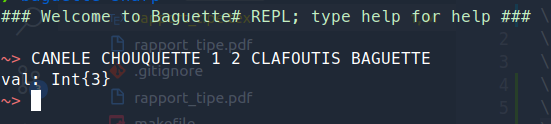
\includegraphics[width=0.6\textwidth]{img/add.png}
        \caption{Résultat dans le REPL de l'opération 1 + 2}
    \end{figure}
    
    La liste des mots clé de définitions est assez courte, il s'agit de \textit{IF,LABEL,GOTO} leur utilisation est expliquée \href{https://www.baguettesharp.fr/advanced.html#labels}{ici}
    à l'exception de ces mots clé, toutes les instructions doivent avoir leur paramètre entre parenthèse, les paramètres peuvent 
    être séparés par une virgule le \textit{lexer} ne les vois pas. Mais ils doivent être séparés par un espace au minimum (y compris avec une virgule)
    \begin{lstlisting}
        CANELE CHOUQUETTE 1 , 2 CLAFOUTIS BAGUETTE
    \end{lstlisting}
    est équivalent à 
    \begin{lstlisting}
        CANELE CHOUQUETTE 1 2 CLAFOUTIS BAGUETTE
    \end{lstlisting}
    Une explication complète de la syntaxe est disponible sur le \href{https://github.com/coco33920/ocaml-baguettesharp-interpreter/wiki/The-basics#syntax}{wiki-syntaxe}
    \subsection{Librairie Standard}
    Une liste complète des instructions est visible sur le \href{https://github.com/coco33920/ocaml-baguettesharp-interpreter/wiki}{wiki}
    et un tutoriel sur l'utilisation basique est disponible \href{https://www.baguettesharp.fr/basic.html}{ici}. La librairie 
    standard du langage implémente les usages suivants :
    \begin{itemize}
        \item Opération Mathématiques sur les entiers et flottant 
        \item Algèbre booléenne
        \item Lecture de l'entrée standard, écriture sur la sortie standard
        \item Manipulation de tableaux 
        \item Manipulation de chaînes de caractère
    \end{itemize}
    \bigskip


    Le langage est typé faiblement, et avec inférence de type, les types primitifs suivants sont implémentés
    \begin{itemize}
        \item Nombres entiers, flottants (NB: aucune distinction n'est faite entre les deux en général)
        \item Chaînes de caractères (NB: les caractère sont des chaînes de caractère de longueur 1)
        \item Booléans (\textit{CUPCAKE} est \textit{true} et \textit{POPCAKE} est \textit{false})
        \item Null (le \textit{unit} de OCaml)
    \end{itemize}
    \bigskip 

    Enfin le langage implémente les tableaux, à savoir qu'ils peuvent être \textit{non-homogène}
    donc vous pouvez faire un tableau contenant deux entiers, trois flottants et quatre chaînes de caractère
    cependant comme ce sont des tableaux ils sont de \textit{taille fixe} et ils héritent du caractère \textit{mutable}
    des tableaux de OCaml

    \section{Machine de Turing Binaire en \bs}
\end{document}